\section{DESENVOLVIMENTO}

\lipsum[2] 

\lipsum[3]

\subsection{TÍTULOS DE SESSÕES}

\subsubsection{Regras}

\begin{itemize} 
    \item Título primário: negrito e em letras maiúsculas;
    \item Título secundário: letras maiúsculas sem negrito;
    \item Título terciário: negrito e com iniciais em maiúsculas;
    \item Título quaternário: iniciais em maiúsculas e sem negrito;
    \item Título quinário: itálico e com iniciais em maiúsculas;
    \item Título sem indicativos numéricos: Caixa alta, negrito, centralizado;
\end{itemize}

Títulos que ocupem mais de uma linha devem ser, a partir da segunda linha, alinhados abaixo da primeira letra da primeira palavra do título.

\newpage

\subsection{SUMÁRIO}

\subsubsection{Exemplo}

\begin{figure}[ht]
    \centering
    \begin{small}
        \caption{Exemplo de um sumário.}
        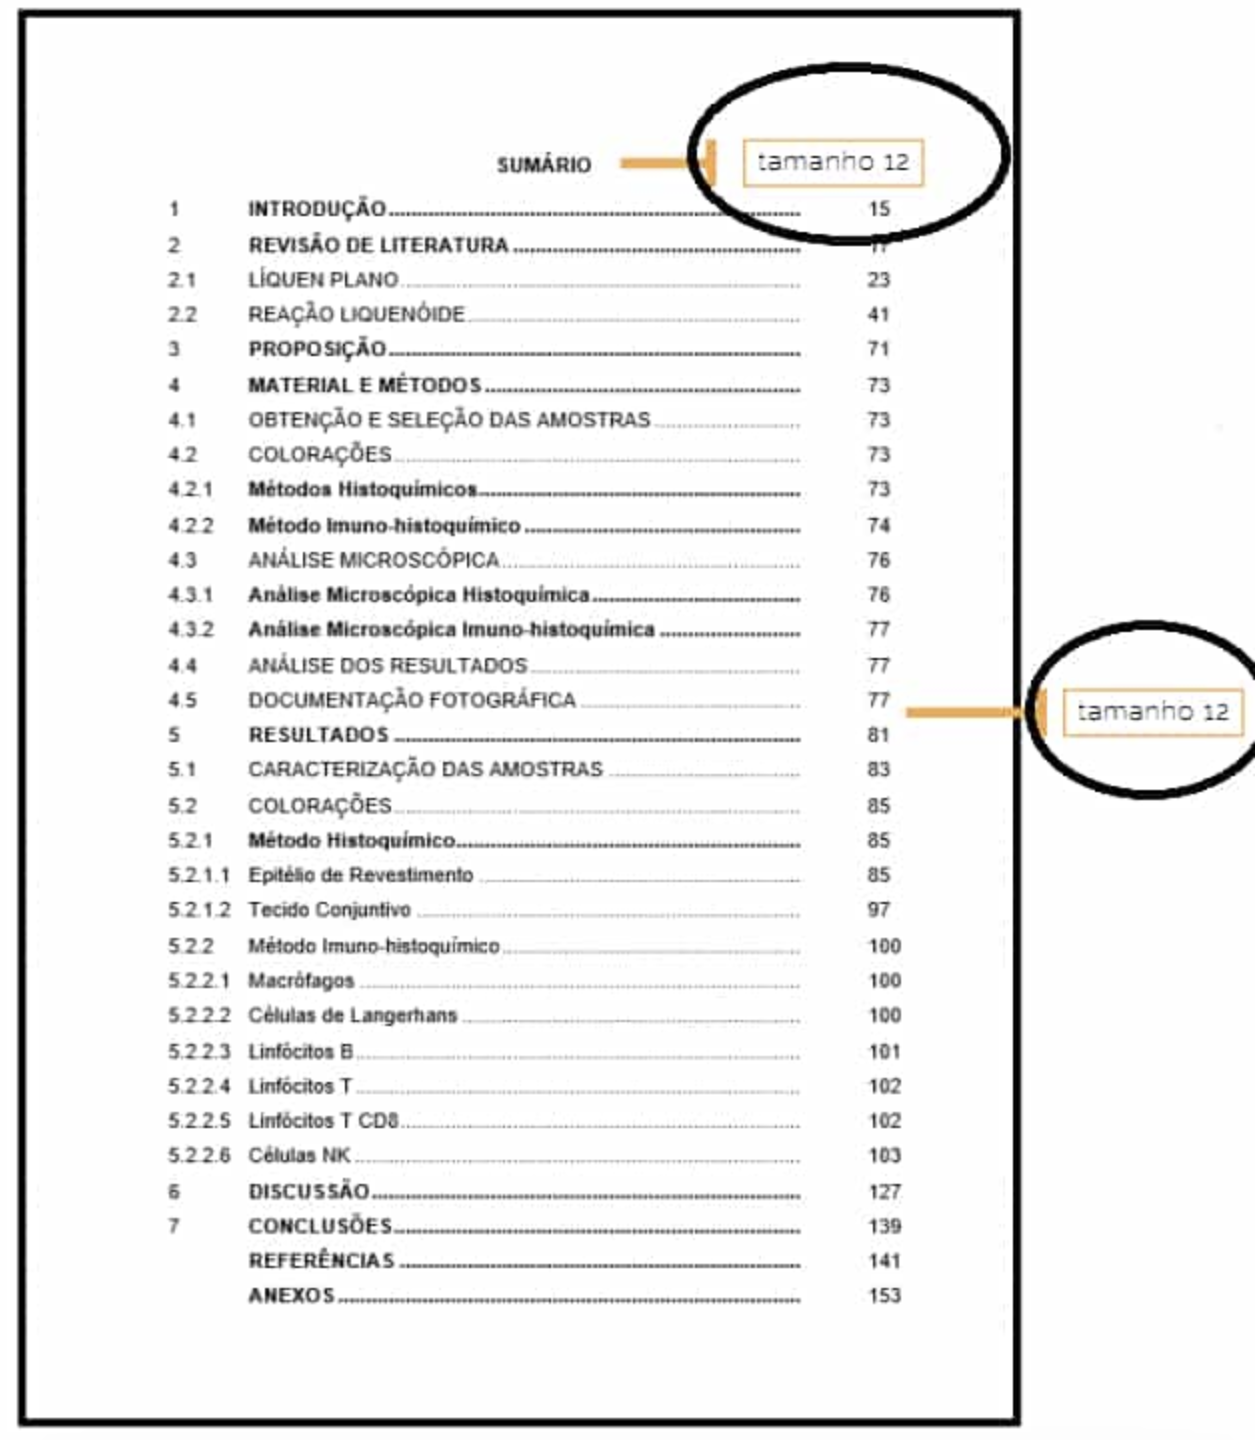
\includegraphics[width=0.9\textwidth]{Figuras/exemplo_sumario.png} % Change to the path of your image
        \label{fig:exemplo_sumario}

        Fonte: elaborado pelo autor (2025)
    \end{small}
\end{figure}

\newpage

\subsubsection{Regras}

\begin{itemize}
    \item A margem superior e esquerda deverá ser de 3 cm;
    \item A margem inferior e direita deverá ser de 2 cm;
    \item O título deverá ficar centralizado e em letra maiúscula;
    \item O sumário deverá ficar antes da introdução;
    \item Você deverá organizar de acordo com os capítulos, seções e partes, tudo na ordem que seu trabalho será!
    \item O sumário deverá ficar depois da capa, folha de rosto, folha de aprovação, dedicatória, resumo ou listas;
    \item A palavra “sumário” ficará no topo da página em negrito, com a mesma fonte e tamanho do resto do texto;
    \item O espaçamento entre as linhas deverá ser de 1,5;
    \item O tamanho da fonte deverá ser 12;
    \item Não deverão conter outros textos, apenas os títulos das divisões e subdivisões;
    \item Os capítulos devem ser escritos com todas as letras em caixa alta, com fonte tamanho 12, em negrito e em alinhamento à esquerda;
    \item Os subcapítulos devem ter a mesma formatação dos capítulos, mas com apenas a primeira letra maiúscula, o resto em letra minúscula;
    \item Os subcapítulos não são em negrito como os capítulos.
\end{itemize}

\newpage

\subsection{IMAGENS}

\subsubsection{Como citar figuras?}

Antes de incluir qualquer elemento visual na sua pesquisa, é importante que você faça a menção no texto. Vamos supor que você pretende incluir uma imagem que mostre o processo de atendimento ao cliente realizado por uma determinada empresa. Isso poderia ser feito da seguinte forma:

''Para atender o consumidor com qualidade, é necessário que a organização tenha um processo de atendimento (figura 1) muito bem estruturado.'' 

 Ou assim: 

``Atender o cliente com qualidade é uma forma de satisfazê-lo e fidelizá-lo. Para isso, é fundamental definir uma metodologia eficiente. A figura 1 mostra o processo de atendimento executado pela empresa xyz.`` 

Depois, você deve colocar a figura centralizada, próxima ao trecho ao qual ela se refere.

\subsubsection{Insira legenda e fonte}

Na parte superior da ilustração, é preciso escrever a legenda para mostrar o que está sendo retratado na imagem. Desse modo, coloque a palavra “figura”, o número que corresponde à ordem em que ela aparece no texto e o título. Por exemplo: 

Figura 1– Processo de atendimento ao cliente da empresa xyz 

Na parte inferior , indique a fonte de onde retirou a figura. Para isso, escreva o termo “fonte”, o sobrenome do autor e o ano de publicação. 

Fonte: Marques (2019)  

Caso você seja o autor da foto, faça da seguinte forma: 

Fonte: elaborado pelo autor (2020) 

\begin{figure}[ht]
    \centering
    \begin{small}
        \caption{Figura de exemplo.}
        
\includegraphics[width=0.3\textwidth]{Figuras/placeholder_photo.jpg} % Change to the path of your image
        \label{fig:exemplo_fig}
        
        Fonte: elaborada pelo autor (2025)
    \end{small}
\end{figure} 

\newpage

\subsubsection{Imagens em LaTex}

Você pode referenciar uma imagem em \LaTeX, usando \verb|autoref| e \verb|label|. Exemplo:

''Para atender o consumidor com qualidade, é necessário que a organização tenha um processo de atendimento (\autoref{fig:exemplo_fig_2}) muito bem estruturado.''

\begin{figure}[ht]
    \centering
    \begin{small}
        \caption{Outra figura de exemplo.}
        
\includegraphics[width=0.5\textwidth]{Figuras/placeholder_photo.jpg} % Change to the path of your image
        \label{fig:exemplo_fig_2}
        
        Fonte: elaborada pelo autor (2025)
    \end{small}
\end{figure}

\subsection{MATEMÁTICA}

You can use mathematical formatting, such as:
\[
f(x) = \int_{0}^{\infty} e^{-x^2} \, dx
\]
or numbered equations like:
\begin{equation}
    E = mc^2
\end{equation}

\newpage

\subsection{FAZENDO REFERENCIAS BIBLIOGRÁFICAS}

Para fazer referencias bibliograficas em LaTex, voce deve usar o comando \cite{dirac} para fazer uma citação à algum artigo mencionado no arquivo \texttt{Referencias.bib}.

% \cite{website:ArduinoLabview}
% \cite{website:OPENSOURCESW}
% \cite{website:OPENSOURCEHW}
